7.-

Consideramos la gramática $G = \langle \Gamma, S, \Sigma, P \rangle$, definida como:

\begin{itemize}
    \item $\Gamma = \{\langle E \rangle\}$ 
    \item $S = \langle E \rangle$ 
    \item $\Sigma = \{a, +, *\}$ 
    \item Reglas de producción $P$:
\end{itemize}
\[
\langle E \rangle \rightarrow \langle E \rangle + \langle E \rangle \mid \langle E \rangle * \langle E \rangle \mid a
\]

a) \textbf{Derivación 1:} Agrupamos la suma primero: $(a + a) * a$

Comenzamos aplicando la regla de la multiplicación en el nodo raíz y luego expandimos el subárbol izquierdo con la regla de la suma:

\begin{enumerate}
    \item $\langle E \rangle \Rightarrow \langle E \rangle * \langle E \rangle$
    \item $\langle E \rangle * \langle E \rangle \Rightarrow (\langle E \rangle + \langle E \rangle) * \langle E \rangle$
    \item Sustituyendo los no terminales por el terminal $a$: $(a + a) * a \Rightarrow a + a * a$
\end{enumerate}

\begin{center}
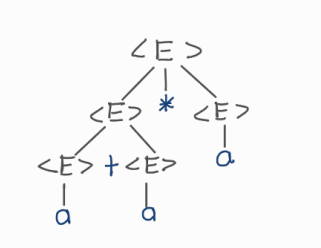
\includegraphics[width=0.5\textwidth]{recursos/arbol1.png}
\end{center}

\textbf{Derivación 2:} Agrupamos la multiplicación primero $a + (a * a)$:

Comenzamos aplicando la regla de la suma en el nodo raíz y luego expandimos el subárbol derecho con la regla de la multiplicación:

\begin{enumerate}
    \item $\langle E \rangle \Rightarrow \langle E \rangle + \langle E \rangle$
    \item $\langle E \rangle + \langle E \rangle \Rightarrow \langle E \rangle + (\langle E \rangle * \langle E \rangle)$
    \item Sustituyendo los no terminales por el terminal $a$: $a + (a * a) \Rightarrow a + a * a$
\end{enumerate}

\begin{center}
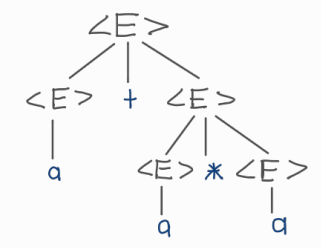
\includegraphics[width=0.5\textwidth]{recursos/arbol2.png}
\end{center}

b) Al existir dos árboles de derivicaión para la misma cadena $w = a + a * a$, podemos concluir que la gramática $G$ es ambigua.
Esto puede ser un problema en el compilador ya que el orden de evaluación de las operaciones deja de ser unico. Al no ver una jerarquía clara puede hacer dos casos:
\begin{itemize}
    \item Si se evalua primero la suma, interpreta la cadena como $(a + a) * a$ 
    \item Si se evalua primero la multiplicación, interpreta la cadena como $a + (a * a)$
    
\end{itemize}
Al poder modificar el orden en el que el compilador evalua las operaciones de una misma expresión se pueden generar resultados distintos.

c)

Definimos la nueva gramática como $X = \langle \Gamma', S', \Sigma, R' \rangle$, donde:

\begin{itemize}
    \item $\Gamma' = \{\langle E \rangle, \langle T \rangle, \langle F \rangle\}$
    \item $S' = \langle E \rangle$
    \item  $\Sigma = \{a, +, *\}$
    \item Reglas de producción $R'$:
\end{itemize}
\[
\begin{aligned}
\langle E \rangle &\rightarrow \langle E \rangle + \langle T \rangle \mid \langle T \rangle \\
\langle T \rangle &\rightarrow \langle T \rangle * \langle F \rangle \mid \langle F \rangle \\
\langle F \rangle &\rightarrow a
\end{aligned}
\]



Para priorizar operaciones, separamos la gramática en niveles : la suma $+$ se queda arriba ($\langle E \rangle$) y la multiplicación $*$ se va más abajo ($\langle T \rangle$). Esto obliga al árbol a resolver siempre la multiplicación antes que la suma.

Al escribir $\langle E \rangle \rightarrow \langle E \rangle + \langle T \rangle$, aseguramos que las operaciones se vayan agrupando de izquierda a derecha sin confusiones.
 
\textbf{Resultado:}
 Para la cadena $a + a * a$, esta nueva gramática solo permite construir un único árbol posible, resolviendo así el problema de la ambigüedad.

